\section{Geometry}

\subsection{Formulas for Area and Perimeter of Geometric Figures}

\begin{itemize}
	\item \textbf{Square}
	      \begin{itemize}
		      \item Area: $A = a^2$
		      \item Perimeter: $P = 4a$
	      \end{itemize}

	\item \textbf{Rectangle}
	      \begin{itemize}
		      \item Area: $A = l \cdot w$
		      \item Perimeter: $P = 2(l + w)$
	      \end{itemize}

	\item \textbf{Circle}
	      \begin{itemize}
		      \item Area: $A = \pi r^2$
		      \item Circumference: $C = 2\pi r$
	      \end{itemize}

	\item \textbf{Triangle (General)}
	      \begin{itemize}
		      \item Area: $A = \frac{1}{2} b \cdot h$
		      \item Perimeter: $P = a + b + c$
	      \end{itemize}

	\item \textbf{Equilateral Triangle}
	      \begin{itemize}
		      \item Area: $A = \frac{\sqrt{3}}{4} a^2$
		      \item Perimeter: $P = 3a$
	      \end{itemize}

	\item \textbf{Isosceles Triangle}
	      \begin{itemize}
		      \item Area: $A = \frac{b}{4} \sqrt{4a^2 - b^2}$
	      \end{itemize}

	\item \textbf{Trapezoid}
	      \begin{itemize}
		      \item Area: $A = \frac{1}{2}(a + b)h$
		      \item Perimeter: $P = a + b + c + d$
	      \end{itemize}

	\item \textbf{Parallelogram}
	      \begin{itemize}
		      \item Area: $A = b \cdot h$
		      \item Perimeter: $P = 2(a + b)$
	      \end{itemize}
\end{itemize}

% Insert Visual Here
% \includegraphics{geometry_shapes_area_perimeter.png} % ← or use TikZ
% \captionof{figure}{Geometric Figures: Area and Perimeter}

\subsection{Formulas for Area and Volume of 3D Geometric Figures}

\begin{itemize}
	\item \textbf{Cube}
	      \begin{itemize}
		      \item Surface Area: $A = 6a^2$
		      \item Volume: $V = a^3$
	      \end{itemize}

	\item \textbf{Cylinder}
	      \begin{itemize}
		      \item Surface Area: $A = 2\pi r(h + r)$
		      \item Volume: $V = \pi r^2 h$
	      \end{itemize}

	\item \textbf{Cone}
	      \begin{itemize}
		      \item Surface Area: $A = \pi r(r + l)$ with $l$ = slant height
		      \item Volume: $V = \frac{1}{3}\pi r^2 h$
	      \end{itemize}

	\item \textbf{Sphere}
	      \begin{itemize}
		      \item Surface Area: $A = 4\pi r^2$
		      \item Volume: $V = \frac{4}{3} \pi r^3$
	      \end{itemize}

	\item \textbf{Square Pyramid}
	      \begin{itemize}
		      \item Surface Area: $A = a^2 + 2a \cdot l$
		      \item Volume: $V = \frac{1}{3} a^2 h$
	      \end{itemize}

	\item \textbf{Triangular Pyramid (Tetrahedron)}
	      \begin{itemize}
		      \item Volume: $V = \frac{1}{3} A_b \cdot h$
	      \end{itemize}

	\item \textbf{Prism (General)}
	      \begin{itemize}
		      \item Surface Area: $A = 2A_b + P_b \cdot h$
		      \item Volume: $V = A_b \cdot h$
	      \end{itemize}
\end{itemize}

% Insert Visual Here
% \includegraphics{3d_geometry_volume_area.png}
% \captionof{figure}{3D Geometric Figures: Surface Area and Volume}

\subsection{Thales' Theorem}

Thales' Theorem states:
If \( A \), \( B \), and \( C \) are points on a circle where the line \( AC \) is the diameter, then the angle \( \angle ABC \) is a right angle.


\begin{align*}
	\angle ABC = 90^\circ \quad \text{if } AC \text{ is a diameter of the circle}
\end{align*}

% Insert Visual Here
% \includegraphics{thales_theorem_diagram.png}
% \captionof{figure}{Thales' Theorem Visualization}

\subsection{Conversion Between Radians and Degrees}

To convert between radians and degrees, use the following formulas:

\begin{align*}
	\text{Degrees} & = \text{Radians} \times \left( \frac{180^\circ}{\pi} \right) \\
	\text{Radians} & = \text{Degrees} \times \left( \frac{\pi}{180^\circ} \right)
\end{align*}

\section*{Geometric Figures with Formulas (2D)}

\subsection*{Square and Rectangle}
\begin{center}
	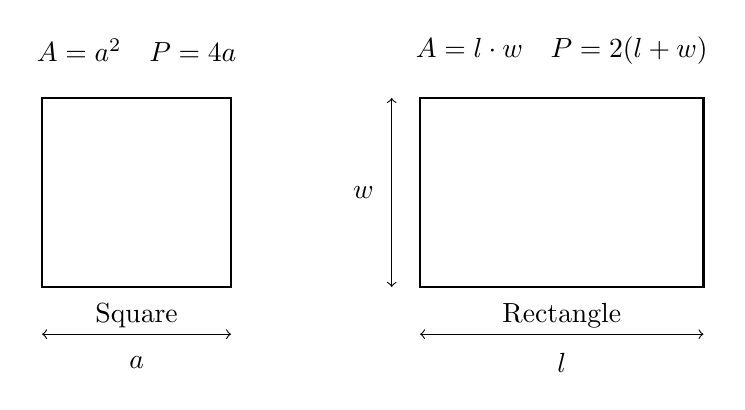
\begin{tikzpicture}[scale=1.2]
		% Square
		\draw[thick] (0,0) rectangle (2,2);
		\node at (1,-0.3) {Square};
		\draw[<->] (0,-0.5) -- (2,-0.5);
		\node at (1,-0.8) {$a$};
		\node at (1,2.5) {$A = a^2 \quad P = 4a$};

		% Rectangle
		\draw[thick] (4,0) rectangle (7,2);
		\node at (5.5,-0.3) {Rectangle};
		\draw[<->] (4,-0.5) -- (7,-0.5);
		\node at (5.5,-0.8) {$l$};
		\draw[<->] (3.7,0) -- (3.7,2);
		\node at (3.4,1) {$w$};
		\node at (5.5,2.5) {$A = l \cdot w \quad P = 2(l+w)$};
	\end{tikzpicture}
\end{center}

\subsection*{Circle and Triangle Types}
\begin{center}
	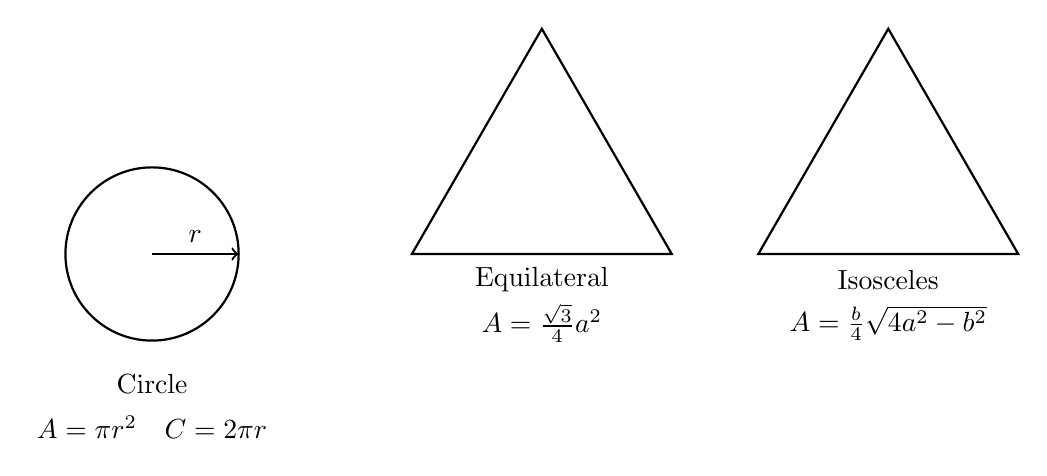
\begin{tikzpicture}[scale=1.1]
		% Circle
		\draw[thick] (0,0) circle(1cm);
		\draw[thick, ->] (0,0) -- (1,0);
		\node at (0.5,0.2) {$r$};
		\node at (0,-1.5) {Circle};
		\node at (0,-2) {$A = \pi r^2 \quad C = 2\pi r$};

		% Equilateral Triangle
		\draw[thick] (3,0) -- (4.5,2.6) -- (6,0) -- cycle;
		\node at (4.5,-0.3) {Equilateral};
		\node at (4.5,-0.8) {$A = \frac{\sqrt{3}}{4} a^2$};

		% Isosceles Triangle
		\draw[thick] (7,0) -- (8.5,2.6) -- (10,0) -- cycle;
		\node at (8.5,-0.3) {Isosceles};
		\node at (8.5,-0.8) {$A = \frac{b}{4} \sqrt{4a^2 - b^2}$};
	\end{tikzpicture}
\end{center}

\subsection*{Scalene Triangle, Trapezoid, Parallelogram}
\begin{center}
	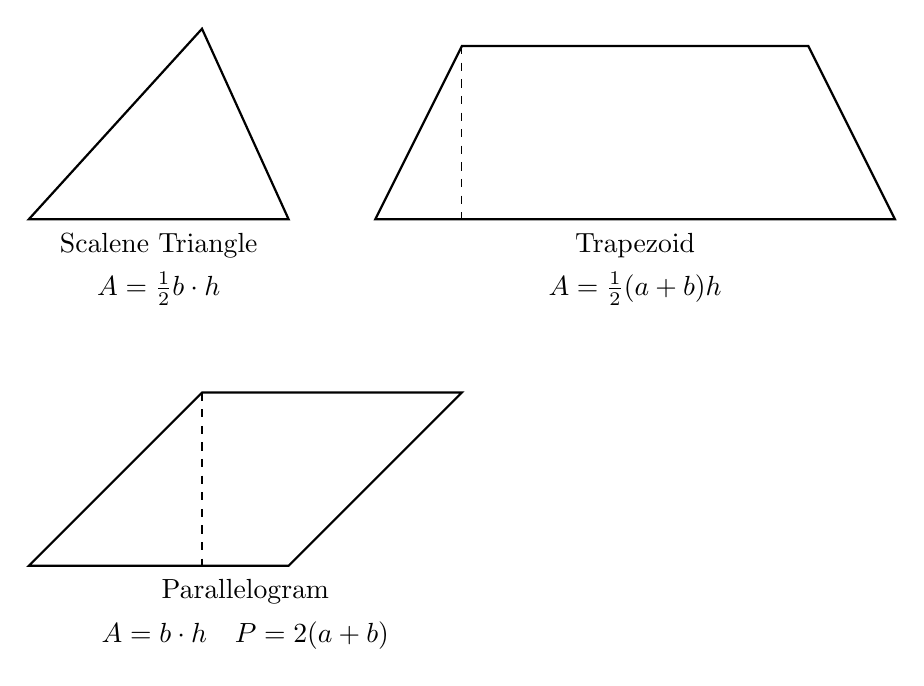
\begin{tikzpicture}[scale=1.1]
		% Scalene Triangle
		\draw[thick] (0,0) -- (2,2.2) -- (3,0) -- cycle;
		\node at (1.5,-0.3) {Scalene Triangle};
		\node at (1.5,-0.8) {$A = \frac{1}{2} b \cdot h$};

		% Trapezoid
		\draw[thick] (4,0) -- (5,2) -- (9,2) -- (10,0) -- cycle;
		\draw[dashed] (5,2) -- (5,0);
		\node at (7,-0.3) {Trapezoid};
		\node at (7,-0.8) {$A = \frac{1}{2}(a+b)h$};

		% Parallelogram
		\draw[thick] (0,-4) -- (2,-2) -- (5,-2) -- (3,-4) -- cycle;
		\draw[dashed] (2,-2) -- (2,-4);
		\node at (2.5,-4.3) {Parallelogram};
		\node at (2.5,-4.8) {$A = b \cdot h \quad P = 2(a + b)$};
	\end{tikzpicture}
\end{center}

\subsection{3D Geometric Figures with Formulas}

\subsubsection{Cube and Cylinder}
\begin{center}
	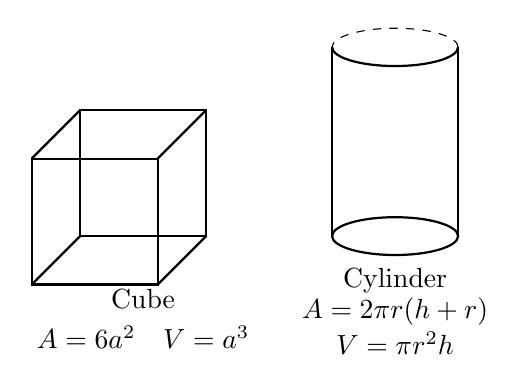
\begin{tikzpicture}[scale=0.8]
		% Cube
		\draw[thick] (0,0,0) -- (2,0,0) -- (2,2,0) -- (0,2,0) -- cycle;
		\draw[thick] (0,0,0) -- (0,0,2);
		\draw[thick] (2,0,0) -- (2,0,2);
		\draw[thick] (2,2,0) -- (2,2,2);
		\draw[thick] (0,2,0) -- (0,2,2);
		\draw[thick] (0,0,2) -- (2,0,2) -- (2,2,2) -- (0,2,2) -- cycle;
		\node at (1,-1) {Cube};
		\node at (1,-1.6) {$A = 6a^2 \quad V = a^3$};

		% Cylinder
		\begin{scope}[xshift=5cm]
			\draw[thick] (0,0) ellipse (1 and 0.3);
			\draw[thick] (-1,0) -- (-1,3);
			\draw[thick] (1,0) -- (1,3);
			\draw[thick] (-1,3) arc (180:360:1 and 0.3);
			\draw[dashed] (1,3) arc (0:180:1 and 0.3);
			\node at (0, -0.7) {Cylinder};
			\node at (0, -1.2) {$A = 2\pi r(h + r)$};
			\node at (0, -1.7) {$V = \pi r^2 h$};
		\end{scope}
	\end{tikzpicture}
\end{center}

\subsubsection{Cone and Sphere}
\begin{center}
	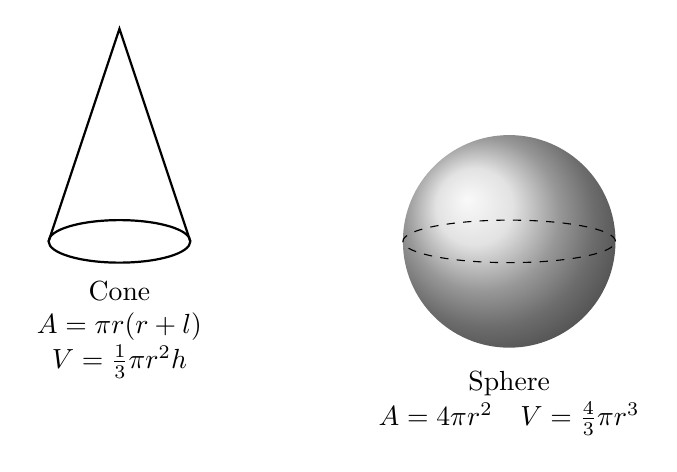
\begin{tikzpicture}[scale=0.9]
		% Cone
		\draw[thick] (0,0) ellipse (1 and 0.3);
		\draw[thick] (-1,0) -- (0,3) -- (1,0);
		\draw[dashed] (1,0) arc (0:180:1 and 0.3);
		\node at (0,-0.7) {Cone};
		\node at (0,-1.2) {$A = \pi r(r + l)$};
		\node at (0,-1.7) {$V = \frac{1}{3} \pi r^2 h$};

		% Sphere
		\begin{scope}[xshift=5.5cm]
			\shade[ball color=gray!30] (0,0) circle (1.5);
			\draw[dashed] (0,0) ellipse (1.5 and 0.3);
			\node at (0,-2) {Sphere};
			\node at (0,-2.5) {$A = 4\pi r^2 \quad V = \frac{4}{3} \pi r^3$};
		\end{scope}
	\end{tikzpicture}
\end{center}

\subsubsection{Pyramid and Prism}
\begin{center}
	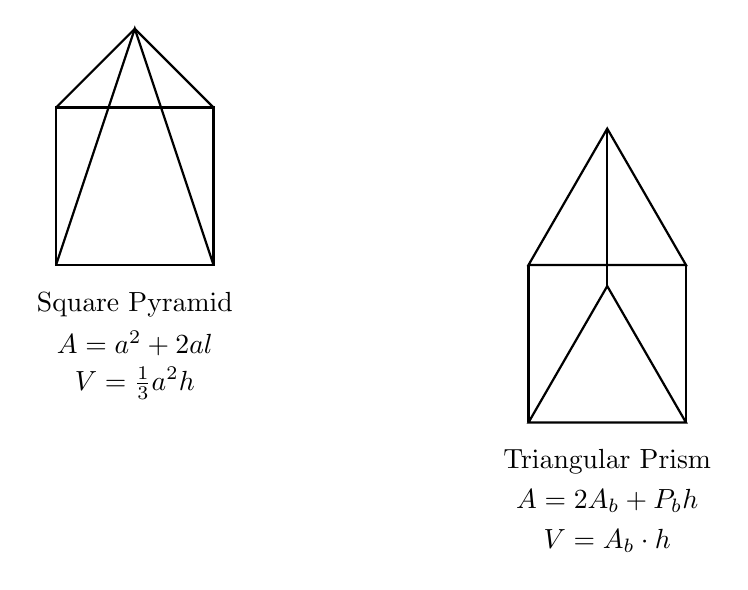
\begin{tikzpicture}[scale=1]
		% Square Pyramid
		\draw[thick] (0,0) -- (2,0) -- (2,2) -- (0,2) -- cycle;
		\draw[thick] (0,0) -- (1,3) -- (2,0);
		\draw[thick] (2,2) -- (1,3) -- (0,2);
		\node at (1,-0.5) {Square Pyramid};
		\node at (1,-1) {$A = a^2 + 2al$};
		\node at (1,-1.5) {$V = \frac{1}{3}a^2 h$};

		% Triangular Prism
		\begin{scope}[xshift=6cm]
			\draw[thick] (0,0) -- (2,0) -- (1,1.732) -- cycle;
			\draw[thick] (0,0) -- (0,-2);
			\draw[thick] (2,0) -- (2,-2);
			\draw[thick] (1,1.732) -- (1,-0.268);
			\draw[thick] (0,-2) -- (2,-2) -- (1,-0.268) -- cycle;
			\node at (1,-2.5) {Triangular Prism};
			\node at (1,-3) {$A = 2A_b + P_b h$};
			\node at (1,-3.5) {$V = A_b \cdot h$};
		\end{scope}
	\end{tikzpicture}
\end{center}

\subsection{Intercept Theorems}

The intercept theorems describe relationships between segment lengths when two rays from a point intersect two parallel lines. They are based on similar triangles and allow us to calculate unknown lengths using proportions.

\subsubsection{First Intercept Theorem}

If two rays start from a common point and are intersected by two parallel lines, then:

\[
	\frac{a}{a'} = \frac{b}{b'}
\]

\noindent where \(a\) and \(b\) are segments on one ray, and \(a'\), \(b'\) are the corresponding segments on the other ray.

\begin{center}
	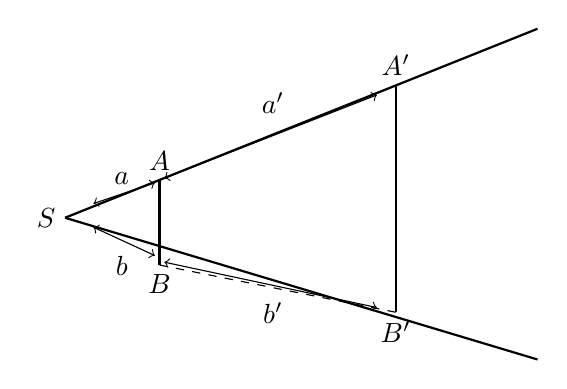
\begin{tikzpicture}[scale=1.2]
		% Rays
		\draw[thick] (0,0) -- (5,2); % upper ray
		\draw[thick] (0,0) -- (5,-1.5); % lower ray

		% Parallels
		\draw[thick] (1,0.4) -- (1,-0.5);
		\draw[thick] (3.5,1.4) -- (3.5,-1);

		% Points
		\node at (-0.2,0) {$S$};
		\node[above] at (1,0.4) {$A$};
		\node[below] at (1,-0.5) {$B$};
		\node[above] at (3.5,1.4) {$A'$};
		\node[below] at (3.5,-1) {$B'$};

		% Helper lines
		\draw[dashed] (1,0.4) -- (3.5,1.4);
		\draw[dashed] (1,-0.5) -- (3.5,-1);

		% Length labels
		\draw[<->] (0.3,0.15) -- (0.95,0.37);
		\node[above] at (0.6,0.25) {$a$};
		\draw[<->] (1.05,0.42) -- (3.3,1.3);
		\node[above] at (2.2,1) {$a'$};

		\draw[<->] (0.3,-0.1) -- (0.95,-0.4);
		\node[below] at (0.6,-0.3) {$b$};
		\draw[<->] (1.05,-0.47) -- (3.3,-0.95);
		\node[below] at (2.2,-0.8) {$b'$};
	\end{tikzpicture}
\end{center}

\subsubsection{Second Intercept Theorem (General Form)}

If a ray intersects two parallel lines, the segments from the origin point to the lines are in the same ratio as the segments along the parallels:

\[
	\frac{SA}{SA'} = \frac{SB}{SB'} \quad \text{and} \quad \frac{AB}{A'B'} = \frac{SA}{SA'}
\]

\begin{center}
	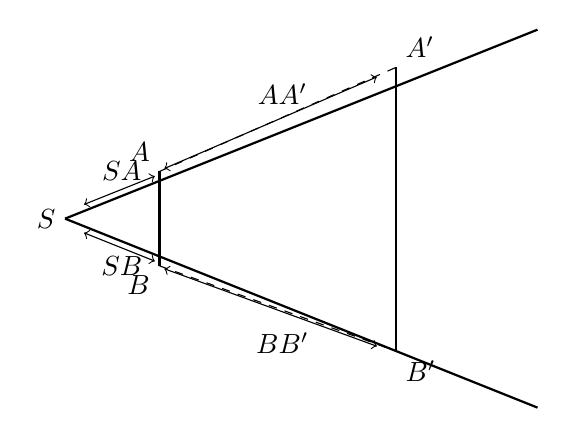
\begin{tikzpicture}[scale=1.2]
		% Rays
		\draw[thick] (0,0) -- (5,2); % upper ray
		\draw[thick] (0,0) -- (5,-2); % lower ray

		% Parallels
		\draw[thick] (1,0.5) -- (1,-0.5);
		\draw[thick] (3.5,1.6) -- (3.5,-1.4);

		% Points
		\node at (-0.2,0) {$S$};
		\node[above left] at (1,0.5) {$A$};
		\node[below left] at (1,-0.5) {$B$};
		\node[above right] at (3.5,1.6) {$A'$};
		\node[below right] at (3.5,-1.4) {$B'$};

		% Helper lines
		\draw[dashed] (1,0.5) -- (3.5,1.6);
		\draw[dashed] (1,-0.5) -- (3.5,-1.4);
		\draw[dashed] (1,0.5) -- (1,-0.5);
		\draw[dashed] (3.5,1.6) -- (3.5,-1.4);

		% Length labels
		\draw[<->] (0.2,0.15) -- (0.95,0.45);
		\node[above] at (0.6,0.3) {$SA$};
		\draw[<->] (1.05,0.53) -- (3.3,1.5);
		\node[above] at (2.3,1.1) {$AA'$};

		\draw[<->] (0.2,-0.15) -- (0.95,-0.45);
		\node[below] at (0.6,-0.3) {$SB$};
		\draw[<->] (1.05,-0.53) -- (3.3,-1.35);
		\node[below] at (2.3,-1.1) {$BB'$};
	\end{tikzpicture}
\end{center}

\newpage

